\chapter{Background}

\section{Search Method}

To support this dissertation, a layered bibliographic search was used.
The first step built a synonym and subtopic list covering grouped and hierarchical time series, telecom anomaly detection, Matrix Profile, combinatorial optimisation, Grammatical Evolution, and anomaly injection, and ran Boolean queries in Google Scholar.
The queries focused on keywords such as ``Multivariate Time Series'', ``Grouped time series'', ``Hierarchical Time Series Forecasting'', ``Hierarchical anomaly detection'', ``Time Series and Anomaly Detection in Telecommunication'', ``Combinatorial Optimization'', ``Anomaly injection'', and ``Matrix Profile''.

Because the combined topic is sparse and hard to retrieve by keywords alone, LLM-based systems were also used to surface additional candidate papers and related terms.
From a small set of highly relevant seed papers, ``Cited by'' and related-work links were followed to catch papers the synonym list missed.

Candidate articles were screened primarily by relevance to the research gap (telecom anomaly detection, aggregation and hierarchy, Matrix Profile and discord detection, combinatorial or evolutionary search, and Grammatical Evolution).
Publication date (preferring work after 2015 where appropriate), venue quality, and citation impact were used as secondary signals, not as a fixed citation cut-off.
Core databases for this stage were IEEE Xplore, Google Scholar, SpringerLink, MDPI, and PLOS.

\section{Time Series}

A time series is a sequence of observations indexed in time order, typically collected at regular intervals (e.g., hourly or daily) \parencite{box2015}.
Irregularly spaced data (e.g., event-driven recordings) can also be treated as time-series data in a broader sense.
Methodological rigor requires consistency in measurement definitions so that observations remain comparable over time.
Time-series data are univariate if they contain a single variable; multivariate series incorporate additional variables while preserving temporal alignment and relevance.

\subsection{Hierarchical Time Series}

Hierarchical time series are structured time-series datasets arranged into hierarchical relationships.
Typical hierarchies include geographical areas (e.g., national $\rightarrow$ state $\rightarrow$ city) or product categories (e.g., product group $\rightarrow$ SKU, stock keeping unit).

Hierarchical time series exhibit multi-level aggregation, where lower-level components combine through arithmetic operations (e.g., summation) to reconstruct higher-level series \parencite{hyndman2021}.
For example, consider a geographic hierarchy:
\begin{itemize}
\item \textbf{Level 1 (National)}: Total sales in a country.
\item \textbf{Level 2 (Regional)}: Sales in the \textit{North} and \textit{South} regions.
\item \textbf{Level 3 (Local)}: Sales in cities (e.g., \textit{North: City A + City B}; \textit{South: City C + City D}).
\end{itemize}
The national series equals the sum of the regional series ($\text{National} = \text{North} + \text{South}$), and each regional series equals the sum of its constituent cities.
This coherence ensures consistency across levels \parencite{wickramasuriya2019}.


As shown in Figure~\ref{fig:hts}, hierarchical time series arrange temporal data into several aggregation levels.
The framework consists of:
\begin{itemize}
    \item \textbf{Root level}: the whole temporal sequence is represented by the aggregate series $y_t$ for $t = 1,\dots,T$;
    \item \textbf{Intermediate levels}: disaggregated elements (e.g., $y_{A,t}$ and $y_{B,t}$) that partition the root series;
    \item \textbf{Leaf level}: the most detailed constituents (e.g., $y_{AA,t}$, $y_{AB,t}$, $y_{AC,t}$ under node A; $y_{BA,t}$, $y_{BB,t}$ under node B).
\end{itemize}

\begin{figure}[H]
    \centering
    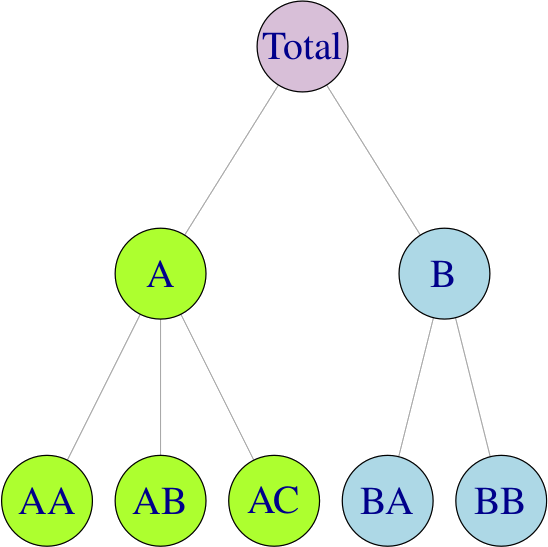
\includegraphics[scale=0.35]{figures/hts.png}
    \caption[A two-level hierarchical tree diagram]{A two-level hierarchical tree diagram \parencite{hyndman2018}.}
    \label{fig:hts}
\end{figure}



\subsubsection{Approaches to Hierarchical Forecasting}

When analysing hierarchical time series, concurrent analysis at several aggregation levels can balance computational efficiency with granularity \parencite{hyndman2018}.


Forecasting within a hierarchical system uses techniques to ensure that forecasts are credible and internally coherent: the aggregation of forecasts at one level should match the forecast of the level above.
The main approaches are bottom-up, top-down, and middle-out \parencite{hyndman2018}.

The bottom-up approach begins its predictions at the base level and aggregates them to higher levels.
This approach is computationally practical and often performs well when upper-level series are relatively stable.
The top-down approach starts at the top of the hierarchy and distributes forecasted totals using historical proportions.
The middle-out approach connects bottom-up and top-down methods by focusing on a mid-level, aiming to balance the strengths of both.

\subsection{Grouped Time Series}

Grouped time series represent collections of temporally structured data organised by shared attributes (e.g., device type, customer demographics) rather than by a single nested hierarchy.
Unlike hierarchical series, grouped data lack inherent aggregation constraints: forecasts for individual series may be developed independently and then analysed collectively for cross-sectional patterns \parencite{hyndman2018}.
Grouped time series are widely used in macroeconomic analysis \parencite{athanasopoulos2017} and supply-chain forecasting \parencite{wickramasuriya2015}, where multiple cross-sectional dimensions demand coherent alignment without a strict hierarchical dependence.

Often, disaggregating factors are both nested and crossed.
For example, Australian tourism data can be disaggregated by hierarchical geographical categories (states, and regions nested within states), but also by four purposes of travel: holiday, business, visiting friends and relatives, and other.
This grouping variable does not nest within any of the geographical variables.
\begin{figure}[H]
    \centering
    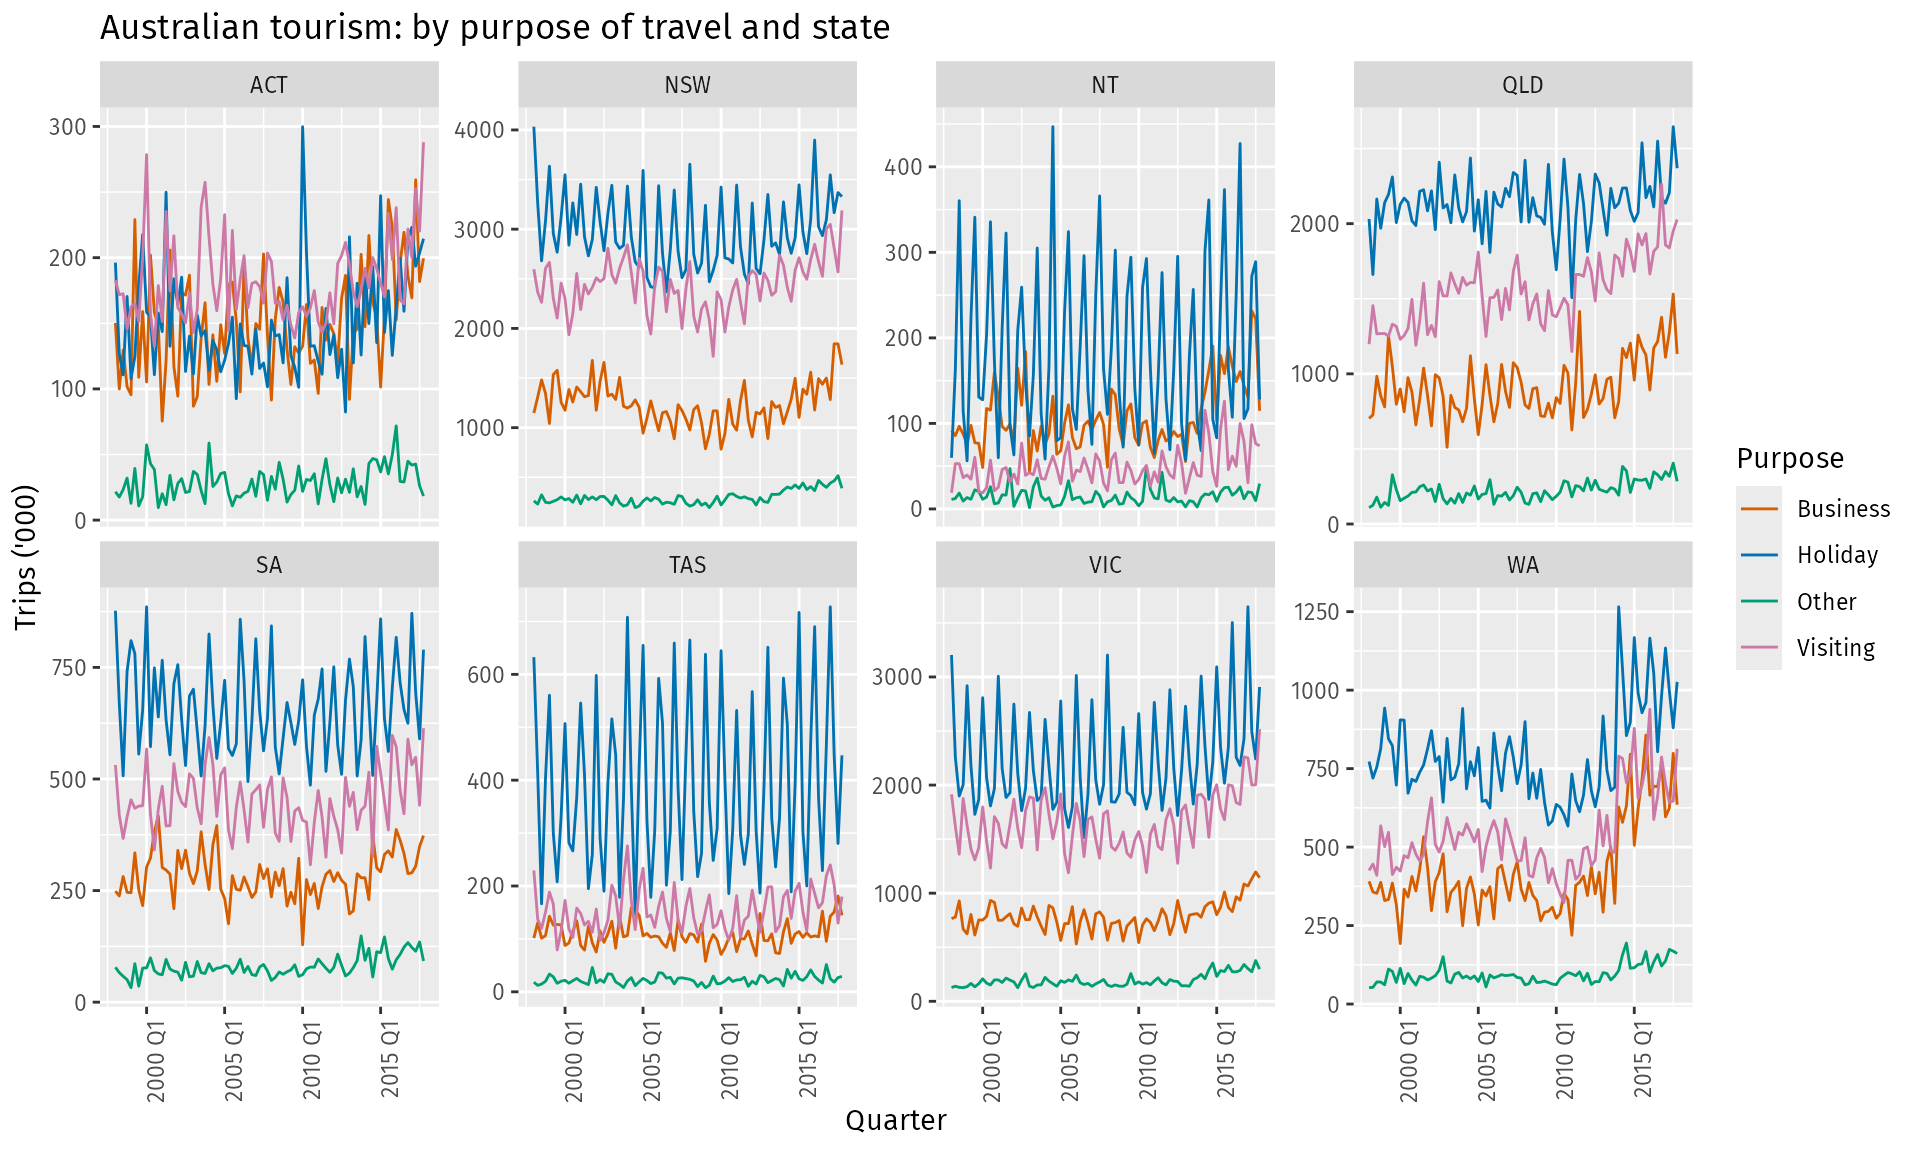
\includegraphics[scale=0.5]{figures/mixed-state-purpose.png}
    \caption[Australian domestic overnight trips, 1998 Q1--2017 Q4, by purpose and state]{Australian domestic overnight trips over the period 1998\,Q1 to 2017\,Q4 disaggregated by purpose of travel and by state \parencite{hyndman2021}.}
    \label{fig:grouped}
\end{figure}

\section{Anomaly Detection}

In machine learning, anomaly detection aims to find patterns that deviate significantly from expected behaviour \parencite{chandola2009}.
It is essential in many fields, including fault diagnosis, network security, and fraud detection.
Univariate anomaly detection identifies outliers in a single variable.
Multivariate anomaly detection considers several variables jointly, so that a point may be anomalous because of an unusual combination of values even when each variable looks normal in isolation.

Anomalies are often classified as point anomalies (a single observation is unusual), collective anomalies (a contiguous subsequence is unusual as a group), or contextual anomalies (an observation is unusual only in a given context) \parencite{chandola2009}.

\subsection{Matrix Profile and Discords}

The Matrix Profile (\ac{MP}) is introduced here because Grammatical Evolution generates many aggregations, and for each produced candidate series a scorer is needed.
\ac{MP} is exact, label-light, and computationally feasible for many candidates.
It takes one candidate time series and computes the nearest-neighbour distance for each subsequence of fixed length, then returns a discord score.

Distance is typically the z-normalised Euclidean distance between two subsequences \parencite{yeh2017timeseriesjoins}: each window is first standardised to zero mean and unit variance, so the comparison is based on shape rather than on the raw level of the series.

A time-series discord is the subsequence most distant from its nearest non-self match \parencite{keogh2005hotsax}.
On the Matrix Profile, the discord is the position with the maximum nearest-neighbour distance \parencite{yeh2017timeseriesjoins}.
For a short and unusual subsequence or spike, the discord may capture well, but may poorly capture a level shift, which is a sustained change to a new level; a ramp, which gradually drifts upwards over time; or a multivariate contextual anomaly, where each series looks normal alone but the relationship is abnormal.

\section{Anomaly Generation}

Anomaly generation is the methodical production of irregular patterns or outliers that depart significantly from normal data distributions \parencite{hawkins1980}.
In machine learning settings it is used both to stress-test system robustness \parencite{chandola2009} and to augment training or evaluation data.
Modern practice emphasises generating semantically plausible contextual anomalies for the target domain \parencite{ruff2021}.

\subsection{Rule-Based Approaches}

Expert-defined constraints in domain-specific anomaly generation deliberately break normal system behaviour \parencite{chandola2009}.
In this dissertation, synthetic anomalies are injected with rule-based thresholds (e.g., values outside $\mu \pm 3\sigma$ over a 168-hour window).

\subsection{Validation of Synthetic Anomalies}

To ensure synthetic anomalies are useful for evaluation, validation typically combines domain checks (e.g., expert judgement that injected patterns are realistic) with quantitative detection benchmarks \parencite{ruff2021}.
In this work, injected labels enable \ac{AUC} evaluation of Matrix Profile discord scores on each candidate aggregation.

\section{Grammatical Evolution}

\subsection{Combinatorial Optimization}

Combinatorial optimisation identifies optimal configurations within finite discrete solution spaces and provides formal frameworks for many NP-hard problems \parencite{papadimitriou1982,garey1979}.
Exact methods (e.g., integer programming, branch-and-bound, dynamic programming) guarantee optimality but can be computationally costly at scale \parencite{papadimitriou1998}.
Approximation and metaheuristic methods---including greedy search, local search, simulated annealing, and genetic algorithms---trade guarantees for tractable near-optimal solutions on large instances \parencite{vazirani2001,glover1989,zlochin2004}.

\subsection{Genetic Programming}

Genetic algorithms evolve a population of candidate solutions by selection, crossover, and mutation.
Genetic programming (\ac{GP}) is a specialised form of genetic algorithm that evolves computer programmes, typically represented as trees whose nodes are functions or terminals \parencite{koza1992}.
An operator of selection uses fitness to choose parents; crossover mixes elements of different parent solutions to produce offspring; mutation introduces random variation; and a survival or replacement operator forms the next generation until a stopping criterion is met.

\begin{figure}[H]
    \centering
    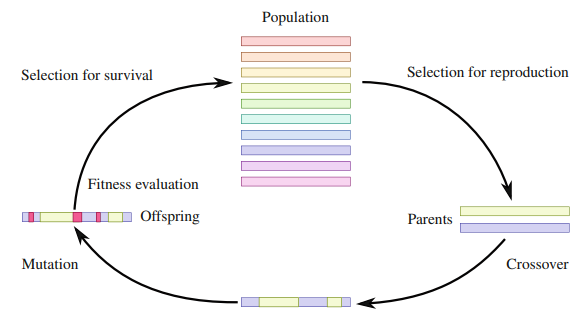
\includegraphics[scale=0.5]{figures/GP_cicle.png}
    \caption[Generational loop in an evolutionary algorithm]{Generational loop in an evolutionary algorithm.
    From a population of solutions, individuals are selected to reproduce by crossover and mutation; offspring are evaluated and incorporated; and a survival operator restores the population size.
    Source: adapted from standard evolutionary-algorithm schematics (see also \textcite{koza1992}).}
    \label{fig:generational_loop}
\end{figure}

\ac{GP} is particularly effective for symbolic regression, automated algorithm discovery, and optimisation tasks \parencite{koza1992,banzhaf2004}.
Population size and the number of generations are crucial parameters that influence exploration of the search space and convergence speed.

\subsubsection{Grammatical Evolution}

Grammatical Evolution (\ac{GE}) is a way to apply evolutionary computing to problems defined by a formal grammar \parencite{oneill2001grammatical,oneill2003}.
A formal grammar is a set of rules that define a language's syntax and allow generation of valid strings or structures.
In \ac{GE}, the genotype is an integer vector rather than a tree; the grammar maps those vectors to valid phenotypes.
This representation supports flexible adaptation to different grammar structures.

The process of Grammatical Evolution involves the following steps:
\begin{enumerate}
    \item Define a \ac{BNF} representation of the grammar;
    \item Randomly generate genotypes as integer vectors;
    \item Evaluate fitness by mapping genotypes to phenotypes and testing them against the fitness function;
    \item Use genetic operators such as crossover and mutation to evolve the population of genotypes;
    \item Repeat steps 3 and 4 until a satisfactory solution is found or a stopping criterion is met.
\end{enumerate}

\subsection{Backus-Naur Form}

A \ac{BNF} grammar describes the syntax of a language as a tuple of four sets:
\begin{itemize}
    \item $T$: the terminal set;
    \item $N$: the non-terminal set;
    \item $P$: the set of production rules;
    \item $S$: the start symbol (a member of $N$).
\end{itemize}

For example, consider a simple grammar for mathematical expressions with addition, subtraction, multiplication, and division, using variables $x$ and $y$:
\[
T = \{+, -, /, *, x, y\}, \qquad
N = \{\langle e \rangle, \langle o \rangle, \langle v \rangle\}.
\]
The non-terminal $\langle e \rangle$ denotes an expression, $\langle o \rangle$ an operator, and $\langle v \rangle$ a variable.
The production rules in $P$ are:
\begin{align}
\langle e \rangle &::= \langle e \rangle \langle o \rangle \langle e \rangle \mid \langle v \rangle \\
\langle o \rangle &::= + \mid - \mid / \mid * \\
\langle v \rangle &::= x \mid y
\end{align}
The pipe operator $\mid$ denotes alternatives.
The start symbol is $S = \langle e \rangle$.

Genotypes may be represented as non-negative integer arrays.
For example, consider
\[
C = [4, 15, 75, 8, 41, 12].
\]
Mapping begins from the start symbol $\langle e \rangle$.
The general rule is
\[
\text{selected\_option} = \text{gene\_value} \bmod r,
\]
where $\text{gene\_value}$ is the current integer from the genotype, $r$ is the number of production choices available for the current non-terminal, and $\text{selected\_option}$ is the (zero-based) index of the chosen production.

The first gene is 4 and $\langle e \rangle$ has two options, so $4 \bmod 2 = 0$ selects $\langle e \rangle \langle o \rangle \langle e \rangle$.
Continuing left-to-right:
\begin{enumerate}
    \item With gene 15, $15 \bmod 2 = 1$ replaces the first $\langle e \rangle$ with $\langle v \rangle$;
    \item With gene 75, $75 \bmod 2 = 1$ replaces $\langle v \rangle$ with $y$;
    \item With gene 8, $8 \bmod 4 = 0$ replaces $\langle o \rangle$ with $+$;
    \item With gene 41, $41 \bmod 2 = 1$ replaces the remaining $\langle e \rangle$ with $\langle v \rangle$;
    \item With gene 12, $12 \bmod 2 = 0$ replaces $\langle v \rangle$ with $x$.
\end{enumerate}
The final expression is $y + x$.

\subsection{Initialization Phase}

Initialisation can be performed on the genome or on the derivation tree.
To control tree depth, this work uses Position-Independent Grow (\ac{PIG}), which generates individuals that tend to fill the allowed depth range: neither systematically too deep nor too shallow.
\ac{PIG} expands non-terminals in random order rather than always expanding leftmost first, and ensures that at least one branch reaches the maximum depth.
This reduces duplicate structures and increases diversity in the initial population.

\subsection{Selection Mechanism}

The selection mechanism chooses individuals from the population to act as parents for the next generation while retaining some randomness to preserve diversity.
This work adopts tournament selection: a number of individuals are drawn at random, the best individual in each tournament is retained, and the process is repeated until the required number of parents has been selected.

\subsection{Variation Operators}

The variation operators explore the search space by modifying genetic material.
The two primary operators adopted in this work are crossover and mutation.

The crossover operator mixes parent genotypes to obtain offspring genotypes.
Variable one-point crossover, which was chosen for this work, swaps the tails of two parents after cut points selected independently in each parent; because the cut positions need not coincide, offspring genome lengths may differ from those of the parents, enabling combination of beneficial traits of different lengths.

Mutation is applied to every child after crossover, using a codon-based integer-flip method.
Here a codon is one element of the genotype vector: an integer flip replaces that codon with another random integer in the allowed codon range.
Each codon is mutated independently with probability
\begin{equation}
    P_{\text{mutation}} = \frac{1}{\text{genome\_length}}.
\end{equation}
In standard PonyGE2 practice this probability is applied over the genome (or over used codons, depending on configuration); the operator itself does not ``know'' which unused trailing genes will later be consumed by wrapping or unused material.

\subsection{Replacement Strategy}

The replacement strategy determines how new individuals enter the population.
This work uses generational replacement with elitism: the best individuals from the previous generation are retained, while the remaining positions are filled by newly generated offspring.
Elitism helps preserve high-quality solutions while the rest of the population continues to explore.

\section{Metrics}

\subsection{Precision and Recall}

In anomaly detection, precision and recall provide complementary perspectives on model performance, especially under class imbalance (e.g., rare fraud cases among many legitimate events).

\subsubsection{Precision}
\label{subsec:precision}

Precision quantifies a model's ability to minimise false-positive classifications:
\begin{equation}
    \text{Precision} = \frac{\text{TP}}{\text{TP} + \text{FP}},
\end{equation}
where $\text{TP}$ denotes true positives and $\text{FP}$ false positives.

\subsubsection{Recall}
\label{subsec:recall}

Recall evaluates how completely positive cases are identified:
\begin{equation}
    \text{Recall} = \frac{\text{TP}}{\text{TP} + \text{FN}},
\end{equation}
where $\text{FN}$ denotes false negatives.

\subsection{Trade-off and Applications}

Raising the decision threshold typically increases precision and decreases recall, and vice versa; the preferred balance is domain-specific.
High recall is paramount in medical diagnostics, where missing a true positive can be severe.
High precision is crucial in spam filtering, where false positives waste user attention.

\subsubsection{F1 Score}
\label{subsec:f1-score}

The F1 score is the harmonic mean of precision and recall:
\begin{equation}
    \text{F1} = 2 \cdot \frac{\text{Precision} \cdot \text{Recall}}{\text{Precision} + \text{Recall}}.
\end{equation}
It provides a single score when precision and recall should be balanced, but can be misleading under severe class imbalance, where \ac{AUC} or precision--recall curves may be more appropriate.

\subsection{Area Under the ROC Curve (AUC)}

The \ac{ROC} curve plots the true-positive rate against the false-positive rate across classification thresholds \parencite{hanley1982}.
The Area Under the ROC Curve (\ac{AUC}) is a common performance metric for binary classifiers under class imbalance \parencite{fawcett2006}.
It measures the classifier's capacity to discriminate between classes.

\subsubsection{Interpretation and Calculation}
\ac{AUC} values range from 0 to 1, where:
\begin{itemize}
    \item 0.5 indicates random guessing;
    \item 1 represents perfect separability;
    \item values below 0.5 suggest inverted ranking.
\end{itemize}

The Wilcoxon--Mann--Whitney statistic provides a non-parametric \ac{AUC} estimate \parencite{hanley1982}:
\begin{equation}
    \text{AUC} = \frac{\sum_{i=1}^{n_+} \sum_{j=1}^{n_-} \mathbf{1}(s_i^+ > s_j^-)}{n_+ \cdot n_-},
\end{equation}
where $n_+$ and $n_-$ denote the numbers of positive and negative instances and $s$ denotes classifier scores.

\subsubsection{Advantages and Limitations}
\ac{AUC} is robust to class imbalance and does not require a fixed threshold \parencite{bradley1997}.
However, it does not capture cost-sensitive decision contexts and can be misleading when ROC curves cross \parencite{lobo2008}.

\section{Literature Review}
\addtocontents{toc}{\protect\setcounter{tocdepth}{1}}

\subsection{Anomaly Detection in Telecommunications Networks}

Telecommunication anomaly detection is difficult because labels are scarce.
Moreover, the industry produces large amounts of data, with few viable labels that can be identified as anomalies.
Often, the problem is not detecting the anomaly but selecting which subsection of the network window to monitor.

\textcite{gonzalez2024one} apply a Dilated Convolutional Variational Autoencoder (DC-\ac{VAE}), a deep model that scores anomalies jointly across several related time series, to mobile-network counters.
They evaluate it on a fully aggregated view where labels are sparse: of 730{,}000 samples, only 9{,}000 were labeled, using a fixed set of 12 features.
Range-based F1 (range-F1) measures overlap between predicted and labeled anomaly intervals rather than isolated timestamps; they report a mean range-F1 of around 52\%, which is only modest.

\textcite{burgueno2020online} indicate that the network they analyzed had 25{,}000 mobile base station coverage areas.
Moreover, for each cell they analyzed 240 hourly \ac{KPI}s, but the study focuses on only 15 of the most important.
Detection is an online threshold state machine (normal / border / anomalous) run at cell level on that manually selected subset; they report capturing almost 80\% of the labeled network anomalies.
From this perspective, manual selection is a bottleneck because the 225 unmonitored features may still contain relevant information; for example, anomalies may occur in an unmonitored signal.

Call Detail Records (\ac{CDR}) and mobile activity records are recognized for analysis in telecom monitoring.
\textcite{sultan2018cdr} report no detection metrics.

\textcite{lemaire2024early} study early detection of urban events from Orange France mobile Network Signalling Data in Paris: cell-level, one-minute counts of network services (calls, SMS, and related signalling).
They use a Signature detector and hand-designed categorical aggregations over these service types, not temporal aggregation.
Against a curated set of documented urban events, their best precision is 28.63\%, with event recall of about 36\% at the corresponding operating point, indicating many false alarms even when the signal is useful.

Existing work assumes a fixed aggregation and therefore may miss anomalies that would only appear under a different grouping.
Automated search is useful when the best aggregation is not obvious in advance; in those papers, there is a fixed review of aggregation, but they do not address how to automate the aggregation of time series.
The next section will be about this topic.

\subsection{Anomaly Detection in Grouped Time Series}

Anomaly detection in grouped time series treats the detector input as a chosen representation, not the whole network.
The dataset is aggregated by related features/entities at the aggregation level, rather than treating a network as a flat collection of features.
It is important because the detection quality is dependent on the aggregation of features, not only the detector.
Across the reviewed studies, datasets, labels, and metrics differ, so reported scores are not directly comparable.

\textcite{mefleh2025beyond} used an unsupervised Mahalanobis distance approach in a telecommunications setting.
They report \ac{AUC} rising from 0.77 on the raw \ac{KPI} features to 0.86 when denominator information is included (for example, attempt counts that normalise ratios), then to 0.93 with adjusted ratios, and finally to 0.99 with learned adjustments.
This result shows that detection quality changes with feature transformation and aggregation.

\textcite{hua2022genad} show that China Mobile wireless base stations share some operational behavior, which GenAD, a generative reconstruction model, can learn and then use to detect anomalies on other stations in the same network.
GenAD was pre-trained on 3{,}000 unlabeled base stations, using multivariate time series features.
Their F1 score is 0.953 (precision 0.910).
That F1 uses point-adjusted segment scoring: if any timestamp inside a labeled anomaly interval is flagged, the whole interval counts as detected, so the score is not a timestamp-wise F1.

In the study by \textcite{oguz2022anomaly}, they simulate a multi-tier network that includes aggregations from the user equipment measurements and classifies the state of each femtocell access point.
Performance changes with the region of interest (\ac{ROI}) radius, signal shadowing, and aggregation methods.
At a 30\,m \ac{ROI} with 2\,dB shadowing, the 1D \ac{CNN} achieved 80.1\% accuracy, but as \ac{ROI} size and the shadowing increase, the accuracy decreases, so this shows that including more observations is not necessarily beneficial when added signals are less relevant or noisier.

Based on the reviewed studies, we can extract that grouping can strongly affect anomaly detection performance.
Although aggregations are selected manually before modeling the relevant \ac{KPI}s, entities, aggregation levels, and spatial boundaries, none of them systematically search for an aggregation structure that best characterizes the anomaly.

\subsection{Anomaly Detection in Hierarchical Time Series}

Hierarchy in anomaly detection is important because an alert such as ``traffic is abnormal'' is not enough for a telecom operator to act on.
The operator must determine whether it affects the entire network, a region or specific cell of the switch, or only one \ac{KPI} category.
So this top-down approach helps break down into smaller branches; although that hierarchy is not necessarily the best aggregation for detecting anomalies.

\textcite{hong2012tiresias} detect and localize anomalies in hierarchical \ac{ISP} call-detail data.
It analyzes customer-care call logs and signaling call records across predefined hierarchies, allowing operators to identify not only that an abnormal behavior occurs but also the level at which it appears.
They found over 94\% of reference anomalies, and separately reported 99.7\% anomaly identification accuracy.
These results were obtained from a fixed additive hierarchy and Holt--Winters spike forecasting.
So the author demonstrates hierarchical localization rather than searching over alternative aggregation structures.
It does not search for alternative partial aggregations or score non-spike discords, which is the gap addressed by this thesis.

On the other hand, \textcite{wolff2022composite} treat anomaly localization as the sequential search problem of a known tree of processes.
Instead of measuring every leaf process equally, their hierarchical dynamic search method first samples aggregate internal nodes and then moves towards the branch most likely to contain an anomaly.
This shows that hierarchy can be an active search space, not merely a reporting structure used after detection.
However, Wolff assumed tree topology is already known, as search is only within it.
This differs from our approach, which uses a \ac{GE} to generate candidate aggregations before applying the anomaly scorer.

\textcite{huang2026hydra} propose HYDRA, a multi-level hierarchy-driven anomaly detector that builds several hierarchy-based views of each series and combines detection signals across those levels.
It ranked first among 40 algorithms across 40 TSB-AD datasets.

\subsection{Matrix Profile and Time-Series Discord Detection}

Chapter~2 defined the Matrix Profile and discords.
What belongs in this chapter is the published evidence that the scorer is fast enough for many candidate series, and whether it has been used on telecommunications data.

Computational efficiency is substantially improved: a refinery time-series self-join is reduced from an estimate of 153.8 days by brute force to 1.2 hours with STAMP/STOMP \parencite{yeh2017timeseriesjoins}.
Also, \textcite{zhu2016matrixprofileii} showed GPU-STOMP could process 100 million subsequences in about 12 days, compared to the estimate of 1585 years for brute force.
STUMPY \parencite{law2019stumpy} gives the practical implementation of this process in Python.
\textcite{vanonsem2023motif} apply Matrix Profile to production \ac{KPI} series from telecom-provider customers of Skyline Communications (25 series), using it for variable-length \emph{motif} discovery rather than discord scoring.
They report the method is about 3--8 times faster than VALMOD; an example series yields both a 288-point (about one day) motif and a 12-point (about one hour) motif in a single distance-matrix pass.
No detection precision, recall, F1, or \ac{AUC} is reported (manual motif checks).
The series to analyse are chosen in advance, so the paper does not search aggregations.

\subsection{Combinatorial Optimisation for Selecting Time Series}

Little published work searches hierarchical aggregation structures.
Feature-selection methods are reviewed here instead because, from an optimisation viewpoint, the problems are similar: both search a combinatorial space of candidates and score each one with a fitness function.
The spaces themselves differ: feature selection chooses a subset of columns, whereas this dissertation searches grammar-constrained hierarchies.

For feature selection, $n$ features give $2^n$ candidate subsets, so exhaustive search is infeasible for large $n$; \textcite{xue2016survey} survey the evolutionary algorithms used for this search, including genetic algorithms, genetic programming, particle swarm optimisation, ant colony optimisation and differential evolution.

\textcite{linares2024evolutionary} use a genetic algorithm (SEISEN) whose fitness is a filter score, the Conditional Dependence Coefficient, to select lagged features for a multilayer perceptron forecaster.
On an electricity dataset, the feature set falls from 7{,}704 to 3{,}813 while \ac{MAE} improves from 207.193 to 194.400, showing that pruning the input representation can improve accuracy.

\textcite{pietron2025adnev} apply a genetic algorithm at three levels to multivariate time-series anomaly detection: it evolves subsets of input series, an autoencoder architecture for each subset, and the network weights, using validation loss as fitness.
On four sensor benchmarks (SWaT, WADI, MSL and SMAP), the resulting ensemble achieves the best point-wise F1 of 14 methods, with a mean of 0.70 against 0.54 for the next best, at a cost of up to 132 GPU-hours per dataset.

\textcite{he2021mining} search subspaces of high-dimensional financial transaction series with a greedy heuristic and an evolutionary $(\mu+\lambda)$ algorithm, scoring each candidate by discord mining.
On real data, greedy search achieves the higher mean average precision (0.86 against 0.72) but is about 15 times slower (1{,}345\,s against 88\,s).

Across these studies, the common pattern is an evolutionary search over a large candidate space with a fitness function evaluated per candidate.
None searches hierarchical aggregation structures, and none combines the search with a Matrix Profile scorer on telecommunications data; this dissertation does both with grammatical evolution.
\addtocontents{toc}{\protect\setcounter{tocdepth}{1}}

